
%==============================================================================
%
%      File:  Master.TEX  (Stored in TEX$LATEX: as UNHTHESIS.TEMPLATE)
%  Language:  LaTeX - Document Preparation System
%      Date:  26/Dec/2005
%    Author:  Maha El Meseery
%             
%
%   This document  is my master thesis on sketch Recognition and understanding
%
%
%        % latex mythesis
%
%------------------------------------------------------------------------------

%    14 Aug 02 Updated document to latex 2e. Also, changed wording 
%              to be consistent with an X windows system.

%    14 Aug 02 Added \includeonly command in comments.



% During the editing process you will not want to view and print the
% whole document. Uncomment the command below so that only the
% chapters that you want to work on are visible.
%\includeonly{ChapterIntroduction}
%\documentstyle[11pt,unhthesis]{report}
\documentclass[11pt,doublespace]{Sketchthesis}


% Extra modules can be added to your document to extend the things
% the Latex can Do. One of these is psfig which allows you to print
% postscript files. You tell Latex to read these packages using the
% \usepackage command:

\usepackage{psfig}
\usepackage{named}
\usepackage{natbib}
\bibliographystyle{plain}
\hyphenation{gno-mon-ly}

\usepackage {graphicx}
\usepackage{subfigure}
\usepackage{longtable}
\usepackage{array}
%\usepackage[T1]{fontenc}
\usepackage[latin9]{inputenc}

%------------------------------------------------------------------------------
%  Preliminary Pages - Fill in the `blanks' noted.
%------------------------------------------------------------------------------

\begin{document}
                                                        % TITLE PAGE
                                                        %======================
\title{Sketch Recognition using Particle Swarm Optimization Algorithm}             % My theses title
\author{Maha Mohammed Nabeel El Meseery}                               % Y name
\prevdegrees{B.S.,Computer  Engineering}       		% Your old degree
\major{Computer Engineering}                            % My current major
\degree{Master of Science}                              % My new degree
\degreemonth{}                                      % When awarded. to be added when known
\degreeyear{}                                      %
%th today or first day of writing  December 26 2005 
%\thesisdate[]                                     % Date of document.
\DOCUMENTtype{Thesis}                                   % or DISSERTATION
\Documenttype{Thesis}                                   % or Dissertation
\documenttype{Thesis}                                   % or dissertation
\maketitle

\providecommand{\tabularnewline}{\\}
                                                        % COPYRIGHT PAGE
                                                        %======================
%\copyrightyear{2009}                                    % Delete these
%\makecopyright                                          % if no copyright
                                                    % APPROVAL                                                         %======================
\thispagestyle{empty}               % Don't do headers or footers.
\newpage                                                             
\begin{center}     
\LARGE  
\textbf{Sketch Recognition using Particle Swarm Optimization Algorithm}\\
\normalsize by      \\ 
\Large  \textbf{ Maha mohamed Nabeel El Meseery}\\
\vspace*{0.4in}        
\normalsize
A Thesis Submitted To the\\
Faculty of Engineering, Cairo University\\
in Partial Fulfillment of the\\
Requirements for the Degree of\\
MASTER OF SCIENCE
in\\
COMPUTER ENGINEERING\\

\end{center}
          
    Approved by\\                                           
Examining Committee:\\
 \makebox[6in]{\hrulefill}\\ 
Professor Nevin Darwish, Thesis Main Advisor\\
 \makebox[6in]{\hrulefill}\\ 
Professor Samia Mashali,Thesis Advisor \\
 \makebox[6in]{\hrulefill}\\  
Assoc. Professor Magda Fayek,Thesis Advisor\\ 
 \makebox[6in]{\hrulefill}\\ 
Professor  Ashraf Abd El Wahab, Member\\
 \makebox[6in]{\hrulefill}\\ 
Professor Mohamed Zaki Abd ElMegeed, Member\\
 \makebox[6in]{\hrulefill}\\ 
  % \\   you need...\\
%\makeapproval                                           %

                                                        % DEDICATION PAGE
                                                        %======================
%\begin{dedication}                                      % Delete these
												                                  % if no dedication
%\end{dedication}                                        % page.

                                                        % ACK. PAGE
                                                        %======================
\begin{acknowledgments}                                 % Delete these if
All praise is due to Allah Who guided me to this. I could not truly have been led aright if
Allah had not guided me.

I would like to convey my sincere appreciation and graditude to my supervisors; Dr. Nevin Darwish, Dr. Magdah Fayek and Dr. Samia Mashali. I would also be very gratuful for dr. Mahmoud fakhr el din for his assitance with my thesis. Thanks for all the time devoted in making constructive comments and suggestions for improving this thesis. 
I thank my family and friends for thier moral and support. I specifically thank, dina said, noha mansour and marwah shafee. Thanks, for being always there when I needed you the most. I hope to express my gratiude to all of you for supproting me and praying for me through all these years. 
 %Finally, I am very grateful to my dear parents, my family, and my friends whom I consider
%as my sisters. I would like to thank particularly Radwa Aboudina, Fatma Nada, Maha
%Nabil, Haidi Badr, and Marwa Kamal. Thank you all for being always there when I needed
%you most. Thank you for believing in me and supporting me through all these years. I think
%without your support and your prayers, none of this work would be accomplished.
%ii
 \end{acknowledgments}                                   %

                                                        % FOREWORD PAGE
%\begin{foreword}                                        %======================
    											                             % Delete these if
%\end{foreword}                                          % no foreword page.

                                                        % OTHER PAGES
                                                        %======================
\tableofcontents                                        % Always needed...
%\listoftables                                           % Delete if no tables.
\listoffigures                                          % Delete if no figures.


%------------------------------------------------------------------------------
%  Document body - Place text into individual include files, such as
%                  as "chap1.tex", or replace each "\include{}" statement
%                  with your actual document text.
%------------------------------------------------------------------------------
\begin{abstractpage}          
% ABSTRACT PAGE
%==============================
% Creates the abstract page.
%   Your text goes here. Just
%   follow the rules given in
%   the LaTeX manual on how to
%   enter/format text using
%   LaTeX commands.   


% didn't finish it all Need some addint
The need for new level of human computer interaction had lead the researchers to attempt improve the current interfaces. Even though the area of research progressed quickly in speech and handwriting systems, gesture and sketch understanding systems are still starting to get noticed. 


Sketch recognition is defined as the process of identifying the symbols the user draws using a single or multiple strokes. Users draw strokes using a pen and the system immediately interprets their strokes into objects that can be easily manipulated. This research uses Particle Swarm Algorithm (PSO) to divide the strokes the user draws into meaningful geometric primitives. These geometric primitives are grouped to formulate symbols which are further identified. Two algorithm are used to divide strokes, the first algorithm \textit{ALgS1} divides stroke to polygons. The second one \textit{AlgS2}, divides stroke to segments of either lines or curves. The research focuses on the effect of PSO segmentations to the sketch recognition systems. The final recognition is achieved using a set of geometrical and global shape properties features. A SVM (support vector machine) classifier is used to correctly identify shapes. 

Experiments were conducted on three different datasets; Hs-DB a benchmark dataset which contains simple presentation symbols, a LD-DB a set of logic design symbols and EL-DB Electrical symbols. Results show that using \textit{ALgS2} to segment stroke improves segmentation than known algorithms. \textit{ALgS1} achieved good performance on EL-DB and Hs-DB but performed poorly on LD-DB due to high number of curves in every symbol. %The segmentation improvement is tested by final symbol recognition accuracy.  

\end{abstractpage}                              % This ends the page.

                                                % CHAPTERS
                                                %==============================
%\usepackage{graphicx}
\chapter {Introduciton}
\pagenumbering{arabic}

Computer research nowadays aimed at facilitating computer human interaction in every way. Pen-based interface gives the user a pencil-paper like feeling that enhances interaction more than the current used keyboard-mouse computer interfaces. However, until now there are hardly any complete pen based computer systems. Generally, Current Pen-Based systems make use of the Pen or stylus to perform the same role as the mouse / keyboard. The minority of such systems are equipped with handwriting or digit recognition that is typically restricted for specific language. 

 Despite the fact that people frequently express their ideas through drawing them there isn't a system that can fully understand those sketches. Lately, only a few researchers were concerned with the problem although it is highly important.  
Firstly, we need to know;
 \textit { What are the main goals of Sketch understanding systems?}

The main goal of sketch understating systems is to build a system that will interpret the sketches the user draw. The systems ought to be natural as possible to provide user with paper and pencil impression. Furthermore, interpreted sketches are expected to transform into objects, which can me manipulated, modeled and/or simulated. 

Sketch here stand for any hand drawn drawing the user draws using digital stylus or similar device. Normally, sketch are composed of smaller segments we call strokes. The time between pen-up and pen-down events identify each stroke.  The strokes are mainly the path of points, which the user path through between the pen-down and pen-up events while using the stylus or similar device. 

Sketch recognition is procedure that will input a sequence of points from user then segment them into clusters of strokes and recognize those clusters to primitive geometric objects and shapes. However, Sketch understanding is transforming the sketch from a group of primitive shapes into comprehendible identified symbols consistent with each other.
% the entire sketched symbols.

\section{Importance of sketch recognition}
\label{sec:ImportanceOfSketchRecognition}

People normally sketch thoughts rather than expressing them linguistically. For instance engineers mostly drafts their early designs using paper and pencil before using CAD tools.  People in general and engineers specially make use of various sketches during design process as instance organizational charts, informal drafting and formal design sketches \cite{}. The sketching process itself go thorough numerous stages. Firstly, early stages with rough drafting designs or notations which are mainly done using paper and pencil. After those primary rough sketches are edited and altered until they are stabilized and finally they are transformed into the computer.


 Paper and Pencil are preferred in design as they offer a remarkable ease in editing and altering the primary rough sketches. Current CAD systems don't give the designer the ease of altering the early designs. Designer had to sketch primary designs on paper and pencil next, the finally design is transferred into computer using a menu CAD system. The process is time consuming and tiring. The need for fast design and development process is driven by the fast growing industries and technology.
 
 A sketch recognition and understanding system will provide a powerful tool to the designers to draw sketch as they usually draw using paper and pencil with the advantages of computer program. Designer needs a normal sketching environment that will provide him facilities in paper interface and the modifying and simulation that is in current CAD systems. 
 
\section{Problems and challenges}
\label{sec:ProblemsAndChallenges}

 Understanding hand drawn sketches may be trivial for humans but it is challenging problem when speaking about computer-based system. Most of the research made on the sketch understanding is achieved for one particular domain or for strictly a set of pre defined symbols. Further, others restrict the user the freedom in drawing which loose the main goals of paper-like-interface systems.  The only few systems that have achieved the desired degree of freedom for the users are extremely computationally expensive.   

The research in the area had faced few problems that will need to be handled to implement an entirely sketch understanding system. The user draws strokes in a spontaneous and ambiguous manner that intensifies the challenges. The first problem is segmenting strokes from the way the user draw it into primitive geometric. Ink parsing is the problem dealing with clustering interpolated strokes and grouping them into symbols. After that, recognizing the symbols from the space the system can identify is the final problem. All those problems must be solved on a real time constrain to maintain an online sketching system if it was a requirement.

The next sections will explain and investigate each of those problems in details.

\subsection{Segmentations}
\label{sec:Segmentations}

Segmentation is dividing the strokes draws into the geometric primitive's as lines, arcs, and ellipses. The strokes as mentioned before are the path of points between pen-down and pen-up events while using a stylus. The processing of those points is done after that to firstly to detect the critical points or vertices. After that the segment is classified as either line, arc, ellipse or circle. The main problem in this process is in detecting the critical and vertices which are points divide strokes into lines and arc. The user draw the lines and arc in an undefined manner which make it difficult for the program to deicide where the user had finish a line and started a new arc or vice verse; Fig [\ref {fig:strokeinterpolation}].


\begin{figure}

		\includegraphics[scale=0.8]{../../neededfiles/Figures/strokeinterpolation.eps}
	\caption[Segmentation error]{The figure shows an arc that the user draw which can be segmented in different ways as a single line or as an arc where a) The stroke users draw  b)interpretation as a single line segment  b) interpretation as an arc.}
	\label{fig:strokeinterpolation}
\end{figure}



		

\subsection{Ink parsing}
\label{sec:InkParsing}

 The clustering of segmented strokes into group of strokes before passing into the next stage this process is called ink parsing. It is simply deciding when a symbols ends and a new symbol begins.  Ink parsing is most important and difficult challenge as grouping of strokes can be done in many ways and configuration, which increase exponentially with the number of strokes. In addition, the ink parsing will affect the next steps of recognizing. The user does not draw the symbol in same order. Moreover, users can draw a sequence of strokes in symbols then leave it to draw another then return again to add segment to symbols so temporal data is helpful but not conclusive.  The user may also draw the same symbols using different orders and methods for example the user can draw a rectangle using single stroke or using two, three or even four strokes. All those factors gather with the sloppy drawing of the user to increase the complexity of the problem.

\subsection{Ambiguities}
\label{sec:Ambiguities}
 	
The major problem of sketch understanding is the high level of ambiguities in the drawing. The user draws strokes that the computer cannot decide if it is arc or line. The nature of hand drawn sketch it self is highly ambiguous even for human eye you may see two drawn you cannot decide if it is square or rectangle.
 The ambiguities in sketch understanding are found at many levels in the system. Firstly, at the segmentation phase where the same user stroke can be interpreted as a ellipse and a circle. Then the symbol recognition as a symbol can have more than one interpolation. Due to the user sloppy drawing the symbols can have more than one interpolation which varies with the domain drawn in it similar problem was faced in handwriting recognition see Fig [\ref{fig:VorU}] but it was handled with knowing information about the context information which may not be the case in sketch recognition. 
 
\begin{figure}	
	\centering
		
\includegraphics[scale=0.85]{../../neededfiles/Figures/VorU.eps}
	\caption[Ambiguities Handwriting ]{The figure shows that the same letter can be interpreted differently in various contexts; first as V in drive or as U in Cut}
\label{fig:VorU}
\end{figure}

The ambiguity problem must be first recognized ambiguities or varicose interpolations of same symbol. After that, resolve those ambiguities is detecting the best correct interpolation of the symbol.  To solve this problem the program must be able to detect the amount of information needed to decide which interpolation of symbols is the best one. 




\subsection{Search space}
\label{sec:Searchspace}


The user drawn symbols can be having more than one interpolation. In addition, those interpolations increase exponentially with the number of strokes the user draw and as the sketch expands the number of interpolation escalate. This intensifies the search space that the program search to resolve the ambiguities and find best interpolation.

\subsection{Real time}
\label{sec:Realtime}


There are mainly three types of sketch understanding system offline \cite{Vibratory8}, online and interactive. Both online and interactive recognition like \cite{incrmentintention41, SmartSketch56} need the processing after each stroke to be real time so the user does not feel the processing.  
                              % The best way to organize your
\chapter{Literature Survey}
\label{sec:survey}
% this will contians only the finished work .... and my comments to view the old survey see the file
%draft_chaptersurvey 
%\section{Introduction }
%\label{sec:Introduction}
The history of pen and sketch based computing goes back to 1963 with Ivan Sutherland's SKETCHPAD \cite{sutherlandsketch}, which used a light pen to draw on the monitor to create circuit diagrams. Current technology and the increase in computing power have increased the abilities of such interfaces and allowed the implementation of fully sketching systems. Over the years, many other sketching based systems have been developed. Through this history most system focused on building the interactive interfaces to assist users while entering information to the computer. To demonstrate our system inspiration we will first present current research in the area of sketch recognition. In Section \ref{sec:preprocessing}, preprocessing and segmentation methods will be discussed in details. Later, symbol recognition methods will be presented and analyzed in Section \ref{sec:symbolrecogntion}. 


% i need to write a history then small introduction to the survey...
%  i have to state that the next  sections will generally group segmentation and symbol recognition task. 
\section{Preprocessing and Segmentation}
\label{sec:preprocessing}
  In a system that supports free hand sketching, sketching should be as natural as possible. This means that the user can draw symbols using single or multiple strokes without constrains. The goal of a sketch system is making the user feel that using the system is nearly the same as using a pencil and paper. But sketches are incomplete drawings that are sloppy and messy, for example figures \ref{fig:Overshootandundershoot} and \ref{fig:overstroked} show examples of messy sketches drawn by users. This led researchers to perform sort of preprocessing before starting the sketch recognition task itself. The next sections explain different preprocessing techniques. 
   
\begin{figure}
	\centering
		\includegraphics[scale=0.7]{../../neededfiles/Figures/Overshootandundershoot.eps}
	\caption[Neat and Sloppy Symbols] {A sloppy and neat versions of symbol \cite{threeproblmes23}.}
	\label{fig:Overshootandundershoot}
\end{figure}

\begin{figure}
	\centering
		\includegraphics[scale=0.7]{../../neededfiles/Figures/overstroked.eps}
	\caption[Example of an over traced stroke]{Example of an over traced stroke \cite{overtraced24}}
	\label{fig:overstroked}
\end{figure} 

 %The preprocessing can be noise removing, stroke beautification or segmentation.  %Because of this 
 Sezgin and Davis \cite{overtraced24} tried to solve the over traced strokes (see Figure \ref {fig:overstroked})using a thinning algorithm. In \cite{meanshift10,domainindependent17}, Yu uses mean shift procedure as a noise remover and preprocessing step to the recognition step. The mean shift procedure is simply shifting the point to the average of its neighborhoods so smoothing out the noise without changing the global structure of data. Gaussian filters was used to smooth curves \cite {Phoenix88}. These procedures may seem to remove noises in the sketch but it often treat vertices as noise which obscure vertex locations. \\
 %% now the third paragraph..... 
Beside points location information (x, y positions) researcher made uses of the extra information from using digital ink. Some as \cite{mulitstroke5,polygonfeedback31} used stroke speed information to detect critical points where it is stated that user slow down at those critical points. Other used curvature and directions data. %Others \cite {MilitaryCOA37,computationalmodel16,polygonfeedback31}, debated on the importance of the extra information and weather the temporal and speed information is significant. 

 Agar et al. \cite{polygonfeedback31} used the timestamp for each point and compute time difference between every two successive point to help him find corners as he argued that it provides more distinct maximum than the speed information. He mentions that the pointing device (for example the mouse) sampling rate is the reason for this phenomena. The points are sampled at regular time intervals while the pointing device is moving. There are no points while the pointing device is stationary. This leads to a nearly constant time difference between samples while the pen is moving and large difference while the pen is stationary. Contrary to speed information, where the user draws with variant speeds which tends to make the speed information include a lot of noise in the data.
  
Sezgin et al.\cite{earlyprocess} used both speed and direction information. Their system gives better results than using only speed or direction information. This is because the speed information tend to be noisy when drawing large symbols, on the other side when using only direction information the some corner are missed. Our system uses speed, direction and time difference information in its preliminary calculation step. This ensures that all the possible vertices are considered when the segmentation algorithm segments strokes. %both speed and direction information help detecting vertices when the 
 


  % third should speech on how systems define critical points (this paragrah should speak on the data collected (speed crital points, ... 

 After critical point detection most sketch system proceeds to label segments into simple geometric primitives (i.e line, arc, etc...).  A hybrid algorithm was introduced in \cite{earlyprocess} where different sets of segments are generated based on both curvature and speed dominant points, followed by choosing a segmentation with the least error from a generated hybrid set. However, this system is limited to recognizing only specific simple geometric shapes with a set of low level recognizers. Each low level recognizer is designed to recognize only one geometric shape using spatial and geometric information extracted from input stroke.  
 
  A genetic algorithm was used by \cite{CruveDivisionSwarm} to optimally divide digital curves into lines and curves. Chen et al. \cite{CruveDivisionSwarm} uses digital curves scanned from paper as input to the system. Also, they did not take advantage of the curvature or local geometric properties of the digital curve. Yin \cite{PolygonApproximationPSO} used PSO to convert digital curves into polygons, our system adopts  Yin \cite{PolygonApproximationPSO} method and tries to improve it by adding curvature and other local information while segmenting strokes to achieve better segmentations. %The next section presents the general particle swarm algorithm which is used in both our segmentation algorithms. % are presented in section \ref{subsubsec:Discreteparticleswarmalgorithm}
 
 
Yu \cite{meanshift10} introduced a \textit{feature area} for each primitive and then computed the segmentation error for different types of primitives based on the computed \textit{feature area}. Figure \ref{fig:featurearearc} shows the feature area of a line and circle in Yu system, the shaded area is the difference between the computed feature area and the assumption area. His system achieved good accuracy in simple shapes (square, ellipse,...etc) but did not perform well in complex shapes. 
 
 Paulson and Hammond \cite{Paleosketch08} introduced a set of low level recognizers that were reported to achieve 98\% accuracy. However, their system similar to all low level recognizers in the way that it identifies a small set of simple shapes.% A genetic algorithm was used by \cite{CruveDivisionSwarm} to optimally divide digital curves into lines and curves. Chen et al.\cite{CruveDivisionSwarm} uses digital curves scanned from paper as input to the system and did not take advantage of the curvature or local geometric properties of the digital curve.
 
Arvo \cite{Fluid25} Tried to combine fast morphing and basic recognition for the sketch drawn as the user draw it. It tries to move the points of strokes drawn by the user draw into one of the known shapes (ex: box, lines and circle). It uses a relaxation and least square method for circles and uses the string of forces for finding best-fit box. However, their system can only identify circle and rectangles drawn using a single stroke.  
\begin{figure}
	\centering
	\subfigure[Feature area of line an arc]{
		\includegraphics{images/featurearearc.eps}}
		\subfigure[Feature area of line]{
				\includegraphics{images/featureareline.eps}}
	\caption[Feature Area]{Feature Area \cite{meanshift10}}
	\label{fig:featurearearc}
\end{figure}

\section{Symbol Recognition}
\label{sec:symbolrecogntion}

%In this section, we review three different types of symbol recognition methods.
 Symbol recognition can be based on: strokes, global shape properties, and appearance \cite{Oltmans07}. The role of which each stroke plays in the structure of the sketched symbol is used to determine shapes in stroke based methods. In global shape properties approach, systems investigate general shape properties and its underlying strokes. Using shape properties relaxes the assumption and role of each stroke in the symbol but it does not truly represent the appearance of the symbol. Unlike appearance based methods where individual strokes are disregarded and they focus on the overall appearance of shapes. We choose to use the method based on shape property but added some geometrical and structure properties used in most stroke based approaches. Our method tries to avoid many of the problems faced by approaches based on individual strokes or global shape properties while trying to gain the additional information that the stroke based system use. In the next sections, we look into three different symbol recognition approaches, describe their advantages and challenges.  

\subsection{Stroke Based Recognition}
\label{sec:StrokebasedRecognition}
Stroke based approach is based on the assumption that each stroke has a specific role in representing the symbol. Stroke based methods examine each stroke as the user draw it to determine its role in the symbol. These methods are suited to interactive interfaces since users expected that system displays interpretation of the symbol after the stroke is drawn or after drawing a group of strokes. The majority of the research in sketch recognition has focused on stroke-based methods because of the corresponding emphasis on interactive interfaces. Most stroke based systems either represent symbols as gestures or   hierarchical shape. 

\subsubsection{Gesture Recognition}
\label{sec:GuestureRecognition}

Single stroke gestures recognition was the focus of the early work in symbol recognition \cite{gestureexample12,aideddesgin22,sketchinginterfaces2}.  Gestures are pen strokes drawn by the user that can immediately recognized by the system. The result was either creating an action (e.g. deleting a shape) or drawing a shape on the screen. These systems are based on how the user draw the shape rather than how it looks. 

One of the first systems in gestures recognition is Rubine's algorithm \cite{gestureexample12} . He used Gaussian statistical classifier to classify gestures.  Simple features as length of stroke, smoothness of stroke, the angle that the first part of the gesture is drawn at and properties of the bounding box of the stroke are used to train the classifier to recognize symbols. In our system, we combine Rubine features with others to include the information on how the user draws sketch while recognizing the symbols. In \cite{Long00}, Long shows how similarities between gestures can be analyzed.  He used this information to identify gestures that are likely to confuse the recognition system. This helped interface designers to choose gestures that are easily recognized. 

The main problem with gesture based recognition systems that they impose several constrains on how the user can draw. Gestures must be drawn using a specific order and direction to be recognized correctly. Moreover, in most cases gestures do not necessarily look like the symbols they represent (e.g. to represent a rectangle the user draws only the left edge of it). Because of these reasons, gestures recognition systems are not suitable for free hand drawn sketches. 

\subsubsection{Hierarchical Shape Descriptions}

A Hierarchical shape descriptions was widely used in sketch systems \cite{sketchunderstanding1,HierarchicalParsing7,Ladder30,AlvaradoFreedom42,napkinGross}. Symbols are represented using hierarchical levels. The lower levels represent simple geometric primitives such as lines, arc and ellipses. Intermediate levels shapes are composed of lower level parts and constrain or connections between them. For example, a triangle is described as three lines connected at their endpoints. Higher level shapes are constructed from intermediate and lower level shapes, for example, a diode is described as a line on the top of a triangle head (acute angle).

 Systems that employ such representation must first pre-process strokes to break them into geometric primitives (see section \ref{sec:preprocessing} for a review on preprocessing methods). Recognition can then be treated as sub graph matching problem.   
 
%Although not based on a formal structural model of shapes, another probabilistic approach by Szummer and Qi in [37] uses conditional random fields (CRFs) to propagate information about the labeling of one stroke fragment to its neighbors. This allows their system to assign labels to stroke fragments that cannot easily be identified in isolation and to regroup over-segmented fragments. This helps mitigate the difficulty of determining the exact granularity at which to perform fragmentation by using the context of surrounding fragments and a global interpretation of the sketch. They have applied their algorithm to the binary labeling problem of distinguishing boxes from connectors in organizational charts with good results, even in several highly ambiguous cases.
\paragraph{Sub-graph matching:}
\label{sec:GraphSearching}

Representing the symbol that the user draws as a graph transforms the classification problem into a graph-matching problem. In general, each user geometrical primitive is represented as a node of the graph and the relations between those nodes are represented as arc. Figure \ref{fig:squarescematic} shows a graph that is constructed by \cite{mulitstroke5} for a rectangle. To classify the symbols the graph constructed must be matched with the graphs in the database. 

\begin{figure}
	\centering
		\includegraphics[scale=0.7]{../../neededfiles/Figures/squarescematic.eps}
	\caption[Semantic Graph of a Square ]{Semantic Graph of a Square \cite{mulitstroke5}}
	\label{fig:squarescematic}
\end{figure}


In the worst case, sub-graph matching is an exponential problem and thus is expensive to compute. Researcher tried to reduce complexity by restricting the search to fragments that are spatially or temporally grouped, or by using other assumptions. Some of the common assumptions are that each stroke is only part of one symbol and that user must draw one shape before drawing the next\cite{physicalmeaning6}. These assumptions add constrains on how user can draw sketches and thus violates freely drawn sketches.  Moreover, the matching process in highly affected by segmentation results. Over or under fragmentation of stroke into geometric primitive complicates the matching process.  If a stroke is broken into too many fragments then there will be extra components that will not map to any part of the symbol. If the stroke is divided enough then there will be component of the shape that are not filled while matching. The different ways of segmenting the sketches worsen the already high cost graph matching. 

 To solve this problem, \cite{mulitstroke5} provided two methods to match graphs, a simpler one using restrictive assumptions and if it fails the system uses a longer more computationally expensive search.  . Figure \ref{fig:squarescematic} shows a semantic graph that is constructed by the trainable recognizer in   \cite{mulitstroke5} for a rectangle. The trainable recognizer construct the semantic network at train time with then match the symbol user draw with the networks in the database. To match the networks quickly the system assumes the user draws the symbol with the same order as in training set. A deep heuristic graph search will employed only if no match was found. % there was no match found.



 Several other systems tried to model the matching process as a probabilistic problem \cite{HMM53,SketchRead2007}. These systems allow matching of partially satisfied shapes to propagate down to re interpret low level fragmentation hypothesis. In SKETCREAD \cite{SketchRead2007}, a dynamically generated Bayesian network represents the shape fragments hypotheses. Higher level structure of shape fragments can cause re interpretation of the geometric primitives. For example, if one head of an arrow is initially labeled as an arc and the system fragments the shape as an arrow then the belief that this stroke is an arc is decrease and the belief that it is a line increase. Finally, the arrow structure is completed and it is fully recognized. 
 
 \paragraph{Visual Descriptive Languages:}
 \label{sec:VisualDescribtiveLanguages}
 
 Avoiding graph matching problems, research tried to use languages that describe shapes instead of graphs. Visual descriptive languages represent the shape with a set of  tokens representing geometric primitives or spatial relations between smaller geometric primitives. Figures \ref{fig:arrow1} and \ref{fig:arr2} show a regular arrow with 2 shafts and head and its definition in Ladder language \cite{Ladder30}. Shape recognition is then a question of parsing the sketch document into a recognizer that parse strokes according to the constructed grammar. 
 
 Several visual grammar were introduced \cite{statisticalparsing26,Ladder30,GenericHMM28}. \cite{Ladder30,GenericHMM28}  Used visual description language which will generate the information of the structure and constrain of each object classified. The system automatically generates Java code for the recognizer for each object. The generated code cycles through the strokes drawn to check if any of the recognizers generated had interpreted any symbols partially or completely.  These systems are less computational expensive than graph matching approach but they also operate based on the output of the segmentation process. Any error in the segmentation process leads to huge error while parsing the whole sketch. Moreover, symbols cannot share strokes between them which influence and restrict how the user draws symbols. 
 % complexity of the graph matching problem 
\begin{figure}
	\centering
		\subfigure[An Arrow]
			{\label{fig:arrow1}\includegraphics[scale=0.75]{../../neededfiles/Figures/arrowladderdef1.eps}}
			\hfill
		\subfigure[Arrow grammar definition]%{\cite{Ladder30}}
		 {\label{fig:arr2}\includegraphics[scale=0.88]{../../neededfiles/Figures/arrowladderdef2.eps}}
	\caption[Arrow Definition]{\cite{Ladder30}}
		\label{fig:arrowladderdef1}
\end{figure}
 
\subsection{Global Shape Properties Based Recognition}
\label{sec:GlobalFeaturesBasedRecognition}

Drawing back from properties of individual strokes several researcher tried to use shape properties on the whole shape to classify shapes. They used global features that try to define the entire shape properties. 

 Several systems \cite{DiagramOfflineConvexHull,MulitStrokeConvexHull} presented features like ratio of bounding box to convex hull area and the ratio of the perimeter to the area.  These global features can be used to distinguish between classes. For example, a rectangle can be distinguished from a triangle by looking to the ratio of area of bounding box to the area of the convex hull. The triangle ratio will be much lower than that of the rectangle. 
 
 Fonseca et al.\cite{Cali63} created a system using similar set of features, their features were used by a number of fuzzy logic rules to identify symbols. They also used Na�ve Bayes model that was trained to classify shapes based on those features. 
 
%Zernike moments were used by Hse et al. in \cite{ToADD}. 
Hse et al. \cite{HeloiseBeautification,zernike61} proposed using the magnitudes of Zernike moments as a shape property. Zernike moments are orthogonal moments which define the distribution of point in the input space. The higher the order of the moment the finer the detail level the point distribution represents. Hse et al. \cite{HeloiseBeautification,zernike61} used a SVM classifier to train the features vector calculated from the moments. Early evaluation of Zernike moments showed that they are invariant to both reflection and rotation of the input shape \cite{ZerMomentOrthogonal}. In our system we used Zernike moments as part of our feature vector. A detailed comparison between Zernike moments and other features are demonstrated in Section \ref{sec:featuresComparisions}. 
 
 
 \begin{figure}[]
	\centering
		\subfigure{Ac Source}{	

		\includegraphics[scale=0.6]{images/acSource.eps}		\label{fig:acSource}}
 
 		\subfigure{Current Source}{	
 		        
		\includegraphics[scale=0.6]{images/CurrentSource.eps} \label{fig:CurrentSource}}
	\caption{Example of Current and AC Sources}
	\label{fig:ACandCurrentSources}
\end{figure}




 
 Systems based on Global shape properties distinguish shapes by learning the different properties each shape class tends to have. These properties do not depend on the order or number of strokes and thus are only based on appearance of the shape not how the user draws it. However, individual details of the shape are impossible to distinguish using these properties. For example, it is impossible to use to differentiate between a current source symbol (circle containing and arrow Figure \ref{fig:CurrentSource}) and a Ac Source (circle containing a wave Figure \ref{fig:acSource}).  Finer details of the symbols are not represented in this approach, thus shapes that have small's details or only significant conceptual variation are not distinguished using this method. These symbols require a system to represent different levels of shape details.  
  
\subsection{Appearance Based Recognition}
\label{sec:ApperanceBasedRecognition}

In the third approach, the recognition focuses on appearance of shapes contrary to individual strokes or global shape properties. Kara \cite{imagetrainable48} used this approach while presenting a system that matches the input shape into a one of the prototypes in the database. Figure \ref{fig:template} shows an example of prototypes of some of the shapes in the system. Input shapes are first pose and scale normalized then four image similarity measures are used to match input shapes to the database prototypes. He used two measures (Hausdor distance) to measure similarity and two coefficients (Yule, Tanimoto) to measure dissimilarity. His approach allows the system to recognize a shape using only a single training sample as it is based on the shape prototype. However, the shape prototype must represent all transformation and variation the input shape can have. Moreover, they restrict the image representation to 48x48 pixels due to computational reasons. This restriction leads to eliminating some of the fine details that may be needed to distinguish some shape classes. There results on isolated symbols seem promising but the system has not been tested on full sketch that tends to have high overlapping between symbols. 
\begin{figure}
	\centering
		\includegraphics[scale=0.7]{images/template.eps}
	\caption[Prototypes of Shapes]{Prototypes of Shapes \cite{imagetrainable48}}
	\label{fig:template}
\end{figure}

\subsection{Discussion}
\label{sec:discuss}

In all of these system only \cite{SketchRead2007} using stroke based recognition have been implemented to the fully create a system that free draw sketch and understand them. This is because the emphasis on the interactive side of the sketch system which result in large difficulties in processing free hand sketches. Methods based on gesture and global stroke properties produce systems that are dependent on assumptions about how strokes can be grouped. These systems assume that users will finish drawing a shape before moving to the next one \cite{multistrokeEvaluation,Cali63,geometrydomain49}. This let them to temporally group strokes and then recognizes them based on their strokes or global shape properties. \cite{AlvaradoDigital} argued that this assumption does not hold in natural sketches. 

Recognition based on strokes using hierarchical shape description is applied in \cite{SketchRead2007}. The principle problem in these systems is the computational complexity of the matching between shape description and geometric primitives produced in the segmentation process. Natural sketch are difficult to segment and group to create reliable fragment of geometric primitives. This is partially due to the increase of noise and other phenomena such as overlapped, over traced strokes and sharing of strokes between different symbols. Since these systems are dependable on the segmentation results, they either perform recognition using undependable segmentation results or consider different ways to segment the input sketch. 

To avoid most problems in such system, our system uses hybrid of both global shape and hierarchical description methods. Currently, our system recognize independent symbols. Each symbol is segmented and hierarchical features are computed.  Features that are representing the global description of the shape are also generated and appended to the hierarchical features. Recognition is done using SVM Linear classifier as it proved to be one of the best learning algorithms. 

\chapter{Particle Swarm Optimization}
\label{sec:ParticleSwramOptimization}

\section{Swarm Optimization Review}
\label{sec:ParticleSwramOptimizationReview}
%This seems to emerge of what is called 'collective intelligence' from often large simple agents.  
% start with swarm in general  .. say about flock , ant and usin in image processing 
% then speeak about PSO and  its firstly generated   (see article)
%mention that is best than ga (see thesis) 

Modeling how a biological swarm has been recently studied by biologist and computer scientists. Scientists in the field of artificial life try to understand how such "social animals" interact, achieve goals and evolve. Moreover, a swarm behavior that achieves some kind of swarm intelligence is increasingly interesting for engineers as they can apply it in optimization. Looking from a higher view, agents in a swarm are cooperating to achieve some purposeful behavior and achieve some common goal. A good example of this cooperation is ant groups looking for food source. A large group of simple independent agents seems to generate this behavior in what is called 'collective intelligence'. Each agent has a set of simple rules to follow, and according to the interaction of the entire group the objective is met\cite{swarmGeneral}. %with other neighbourhood agents. 

Reynolds \cite{swarmflock} created 'boid' which simulated the motion of a flock of birds. Each boid is a simple agent that navigates according to his perception and a set of basic rules.  Kube and Zhange \cite{antsimulation} introduced a simulation model for ant's behavior and used in cooperative transportation. Ants leaves a trail of its movement, so when an ant find food it cannot carry alone, it can easily trace back to the colony and then a group of ants can track the trail and bring the food back.   Kube and Zhange \cite{antsimulation,swarmGeneral} system seems to correctly models ants behavior with a methods of task modeling. 

Image processing is one of the disciplines that used Swarm Intelligence. Ant colony was widely used to segment objects in \cite{antSegmentation,antthreshold,SwarmMedical}. Since 1995 when Kennedy and Eberhart \cite{PSOFirst,PSO2} introduced particle swarm algorithm (PSO) the algorithm had been used in various image processing system as an optimization  algorithm \cite{SwarmImageProcessing,Swarmimageprocessing2,Colorquantization,SwarmMedical}.  PSO algorithm was used in \cite{ToADD} to classify pixel to simplify the object segmentation process. 
 
\section{Discrete Particle Swarm Algorithm}
\label{sec:ParticleSwarmAlgorithm}
%\section{Particle Swarm Algorithm}
%\label{PSO}
%What is particle swarm algorithm and how it was used in related researches. 
The main idea of \textit{Particle Swarm Algorithm (PSO)} is to represent each agent with a particle from the solution space \cite{PSOFirst}. Each agent moves the particle with a direction and velocity $v_{ij}$ based on equations \ref{eq:Swarm} \& \ref{eq:Swarm1}.
\begin{equation}
%\[
p_{ij}=p_{ij}+v_{ij},
%\
\label{eq:Swarm1}
\end{equation}
where $p_{ij}$ represent the $jth$ particle in the $ith$ agent and $v_{ij}$ is the velocity of the $jth$ particle in the $ith$ agent.
 %Equation [\ref{eq:Swarm}] shows how velocity and direction of each particle are computed
 \begin{equation}
v_{ij}  = v_{ij}  + c_1 r_1 (lbest_{ij}  - p_{ij} ) + c_2 r_2 (gbest_{ij}  - p_{ij} )
\label{eq:Swarm}
\end{equation}
 where $lbest_{ij}$ is the local best particle, $gbest_{ij}$ is the global best particle, $r_1$ \& $r_2$ are random variables and $c_1$ \& $c_2$ are the swarm system variables.
 After each iteration the global best $g_{best}$ particle and the agent local best $l_{best}$ particle are evaluated based on the maximum fitness functions of all particles in the solution space. The solution is found after achieving a specific number of iteration or after an error threshold is achieved.
Equation \ref{eq:descrite} is used to change the general swarm algorithm into binary particle (\textit{Discrete Particle Swarm Algorithm DPSO}) which handles particle values of either $0$ or $1$ \cite{PSODisceret}. 
 \begin{equation}
   P(i)\Leftarrow 
\{
\begin{array}{c} 
1 \quad \quad if\quad r_{3}>p_{i}  \\

0 \quad \quad if\quad r_{3}<p_{i} 
\label{eq:descrite}
\end{array}\}
\end{equation}
 where $p_{ij}$ is the numerical values of the particle and $r_{3}$ is a random variable.
  
                              % document is probably to keep
\chapter{Proposed System for Sketch Understanding}
\section{Aims of the System}
\label{sec:AimsOfTheSystem}
The previous chapter shows the current trends in sketch recognition. This thesis introduce a solution for the problem that give optimize solution for the segmentation problem. 

\section{An Overview of the System}
\label{sec:AnOverviewOfTheSystem}
 
 
 
\section{System Components}
\label{sec:SystemComponents}
% the system and discription of this 



\chapter{Preprocessing and Segmentation}
\label{sec:Preprocessingandsegmentation}


\section{Preprocessing}
\label{sec:Preprocessing}

\subsection{Curvature Calculation}
\label{sec:CurvatureCalculation}

\subsection{Critical Point Detection}
\label{sec:CriticalPointDetection}


\section{Segmentation}
\label{sec:Segmentation}
\subsection{Swarm Introduction}
\label{sec:SwarmIntroduction}


\subsection{Ellipse Detection }
\label{sec:EllipseDetection}


\subsection{Swarm Segmentation}
\label{sec:SwarmSegmentation}
\subsubsection{Problem Formulation }
\label{sec:ProblemFormulation}

\subsubsection{Fitness Computation }
\label{sec:FitnessComputation}
\subsubsection{Polygon Division Algorithm}
\label{sec:PolygonDivisionAlgorithm}

\subsubsection{Curve Divisions Algorithm}
\label{sec:PolygonDivisionAlgorithm}


\section{BenchMarck algorithm}
\label{sec:BenchMarckAlgorithm}


\chapter{Symbol Recognition}
\label{sec:SymbolRecognition}
\section{Stroke Clustring Algoirthm }
\label{sec:ClustringAlgoirthm}
\section{ Feature Extraction}%%Feature Set
\label{sec:FeatureExtraction}









%%%%%%%%%%%%%%%%%%%55555555
%Symbol Recognition 16
%4.1 Preprocessing and segmentation . . . . . . . . . . . . . . . . . . . . . . . . . . . 16
%4.2 Feature-Based Statistical Symbol Recognition . . . . . . . . . . . . . . . . . . . . 18
%4.2.1 Feature Set . . . . . . . . . . . . . . . . . . . . . . . . . . . . . . . . . . 19
%4.2.2 Training . . . . . . . . . . . . . . . . . . . . . . . . . . . . . . . . . . . . 21
%4.2.3 Recognition . . . . . . . . . . . . . . . . . . . . . . . . . . . . . . . . . . 23
%4.2.4 User Study . . . . . . . . . . . . . . . . . . . . . . . . . . . . . . . . . . 24
%4.3 Graph-Based Symbol Recognition . . . . . . . . . . . . . . . . . . . . . . . . . . 28
%4.3.1 Previous Work . . . . . . . . . . . . . . . . . . . . . . . . . . . . . . . . 28
%4.3.2 Statistical Graph Definitions and Error-driven Stochastic Graph Mathcing . 29
%4.4 Image Based Symbol Recognition . . . . . . . . . . . . . . . . . . . . . . . . . . 30
%4.4.1 User Study . . . . . . . . . . . . . .
%3.3 System Components 43
%4 Segmenting a Freehand Sketch
%4.1 Interface 51
%4.2 Spline representation 52
%4.3 Points of potential feature separation 59
%4.4 Corner detection 59
%4.5 Intersection detection 61
%4.6 Clustering of interesting points 65
%4.7 Feature Extraction

\chapter{Evaluation}
\label{sec:Evaluation}
This chapter describes and illustrates the experiments performed on the system. In the chapter, section \ref{sec:ExperimentsSetup} describes the experimental setup. Section \ref{sec:Datasets} describes the datasets used. Section \ref{sec:ResultsDetails} demonstrates and analyzes the results. 

The system has two main parts the DPSO stroke segmentation and symbol recognition. Each part is evaluated separately. The preprocessing procedures and computation is evaluated using their effect on the segmentation algorithm. These results are reported in section \ref{sec:ResultsDetails}. The effect of number of agents, the error thresholds and various other PSO parameters are investigated in Section \ref{sec:PSO}. %The results presented in Section \ref{sec:ResultsDetails} and \ref{sec:PSO}.  

The recognition system evaluation is presented in Section \ref{sec:SegmentationAlgorithms}. The recognition rate (computed as the number of correctly recognized samples divided by the total number of samples in the test) for each segmentation algorithm compared to another segmentation algorithm are reported in \ref{sec:recognitionAlgorithms}. Next, a comparison between different shapes and datasets and it influence on the recognition rate is presented in Section \ref{sec:EffectsofSymbolComplixity}. Finally, a comparison between different feature vectors is reported in Section \ref{sec:featuresComparisions}.

\section{Datasets}
\label{sec:Datasets}
Two different data set were used, 
%For classifier and algorithm testing the system used a data set collected by
\begin{description}
	\item [Hse Dataset] (denoted as Hs-DB) Data set collected by \cite{HeloiseBeautification} and was previously used by \cite{Oltmans07} as benchmark for sketch recognition problem. The data are drawn by 16 users each of them have drawn from 30 to 50 samples for each shape. Figure \ref{fig:symbolSet} shows the shapes used in the data set. The dataset was divided into training set and test set. Four different splits for the training and test data are generated from the dataset. In worth noting that \cite{HeloiseBeautification} and \cite{Oltmans07} achieved 96.7\% and  94.4\%  on this dataset respectively. %, 94.4\%  , which
%is comparable to the 96.7%  %The results displayed are the average recognition accuracy of the four splits resulted from the classifier after recognizing the symbols.
		\item [Multi Domain Dataset] (denoted as MD-DB) A dataset we collected manually from different users. The dataset contains symbols from three different domains ( UML, mechanical and electrical engineering symbols). Data are collected from 4 different users each of them have drawn from 20 to 40 samples of each shapes. Figures \ref{fig:LogicSet} and \ref{fig:ElectSet} show some of the shapes used in the dataset. Symbols from different domains were gathered to evaluate the system throughout different types of shapes. Users were requested to draw symbols without any restriction on style, size or orientations. The dataset was divided into training set and test set. Four different splits for the training and test data are generated from the dataset. %The results displayed are the average recognition accuracy of the four splits resulted from the classifier after recognizing the symbols. 
\end{description}
 %We divided the dataset equally into training set and test set.  The results displayed are the recognition accuracy resulted from the classifier after recognizing the symbols. \\
%We divided the dataset into four sets each set contains four different users. Furthermore, each set is divided into train and test set where the trained set where used to train the classifiers and the test set where used for testing.  The algorithms are then tested using the four sets and the results are averaged.
\begin{figure}[]\centering
\fbox{  \parbox{8cm}{% 
		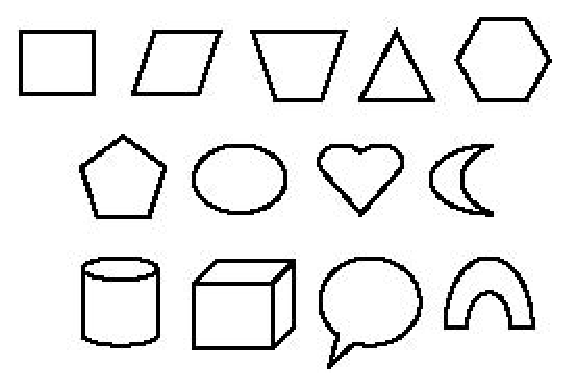
\includegraphics[scale=0.7]{images/symbolSet.eps}	}
		}
	\caption{The Symbol Set}
	\label{fig:symbolSet}
\end{figure}

\begin{figure}[]\centering
\fbox{  \parbox{6cm}{% 
		\includegraphics[scale=0.7]{images/logicSymbols.eps}	}
		}
	\caption{Example of Logic Symbols}
	\label{fig:LogicSet}
\end{figure}
\begin{figure}[]\centering
\fbox{  \parbox{8cm}{% 
		\includegraphics[scale=0.7]{images/SymbolsElectricalr.eps}	}
		}
	\caption{Example of Electrical Symbols}
	\label{fig:ElectSet}
\end{figure}



%\section{Evaluations techniques}
%\label{sec:EvaluationsTechniques}
%\section {Curvature estimation results}
%\label{sec:Curvatureestimationresults}
\section{Performance Measures }
\label{sec:PerformanceMeasures}

\begin{description}
	\item[Segmentation Error] The segmentation error is computed from each stroke after segmentation as computed from in $E_{alg}$ in Equation \ref{eq:bestFit2}. The error represents the sum of Square Root Error of the length from the point on the stroke to the estimated curve or line. 
	  
	\item [Recognition accuracy] We measure recognition performance for each algorithm by determining the number of correctly identified symbols in the whole dataset. Note that All the results are shown as the average of the four split of the dataset used. 
\end{description}

 

\section{Results}
\label{sec:ResultsDetails}

\subsection{PSO Algorithm}
\label{sec:PSO}

Figure \ref{fig:SegErrPreCal} shows the \textit{Average Segmentation Error} using different preliminary calculation (Section \ref{sec:CurvatureCalculation}). The figure shows that using all computations (time difference, direction, speed and curvature) for each stroke decrease the Segmentation error. Figure \ref{fig:PossibledpPreCalculation} shows the average number of Possible dominant point $P_{pd}$ with respect to information used in the system. The results shows that the using all information increases the number of Possible dominate point $P_{pd}$ which in segmentation stage decreases the \textit{Segmentation Error}. It is worth noting that when using all information the number of Possible dominant point $P_{pd}$ is not the same as the sum of using every information alone. This is because we found out that there was some redundant points found using more than one information source.  


   
\begin{figure}
	\centering
		\includegraphics[scale=0.5]{results/SegErrPreCal.eps}
	\caption{preliminary calculation effect}
	\label{fig:SegErrPreCal}
\end{figure}
 
 
\begin{figure}
	\centering
		\includegraphics[scale=0.5]{results/PossibledpPreCalculation.eps}
	\caption{Possible Dominant Point Count}
	\label{fig:PossibledpPreCalculation}
\end{figure}

	 	
 The effect of number of agents, the error thresholds and various other parameters was investigated. The result of these tests are shown in Figure \ref{fig:swarmtestingS1} and \ref{fig:swarmtestingS2}. Figure \ref{fig:swarmtesting} shows that as the number of agents increase the \textit{Segmentation Error} value decrease. Similar results for the maximum swarm iterations are shown in Figure \ref{fig:swarmtesting1}.  Other algorithm parameters like $c_1$,$c_2$ that were mentioned in Section\ref{sec:ParticleSwarmAlgorithm} are tested using similar tests (Figure \ref{fig:swarmtesting} and \ref{fig:swarmtesting2}). The final values are for maximum number of iteration = 80 with 15 particles. The final number of agents and maximum swarm iteration used in the system was based trade off between errors achieved versus the computation time. 
   
   
    
 \begin{figure}
	\centering		
	 \includegraphics[scale=0.3]{results/swarmalg1.eps}
	 	\caption{Segmentation Error Vs. Maximum iterations For ALgS1}
	 	\label{fig:swarmtestingS1}
	%\caption{Experiments results :} a)    b) c) 
\end{figure} 


    
 \begin{figure}
	\centering		
	 \includegraphics[scale=0.3]{results/swarmalg2.eps}
	 	\caption{Segmentation Error Vs. Maximum iterations For ALgS2}
	 	\label{fig:swarmtestingS2}
	%\caption{Experiments results :} a)    b) c) 
\end{figure} 


%The fig. \ref{fig:dataerrorvsiteration.jpg} display the effect of the size of swarm population on the number of vertex reported while segmenting the stroke.\footnote{The fewer the vertex the better the segmentation} The graphs shows that as the number of iteration increase there is a decrease in error until the error reach a saturation and any increase in number of iteration does not affect the error calculated. Similar behavior is noticed in fig. \ref{fig:datapopulation.jpg}.  These curves and test result in choosing the swarm parameters $c_1,c_2$ and maximum number of iteration and the swarm population. The final values are for maximum number of iteration = 150 with 15 particle for better compensation in the time domain. 

%\begin{figure}
%	\centering
%		\includegraphics[scale=0.8]{images/dataerrorvsiteration.jpg.eps}
%	\caption{Error vs. iterations }
%	\label{fig:dataerrorvsiteration.jpg}
%\end{figure}
%\begin{figure}
%	\centering
%		\includegraphics[scale=0.8]{images/datapopulation.jpg.eps}
%	\caption{Swarm Population }
%	\label{fig:datapopulation.jpg}
%\end{figure}


\subsection{Segmentation Algorithms}
\label{sec:SegmentationAlgorithms}
The result of the segmentation algorithm can be viewed in the Figure \ref{fig:results1}. This result shows the originals stroke and the segmentation that the system generated for the stroke. Figure \ref{fig:results2} shows the result of \textsl{AlgS1} and \textsl{AlgS2} for the same input strokes.  Figure \ref{fig:results3} shows the output of \textsl{Alg3} to the same set of input strokes. It clearly shows that \textsl{AlgS2} have better segmentation results than both \textsl{AlgS1} and \textsl{Alg3} but since these segmentation are subjective to what the user intended to draw the next section will focus on the effect of the segmentation algorithm on the recognition accuracy. 

\begin{figure}

	\centering
				\subfigure{\includegraphics[scale=0.55]{results/result1.eps}}
					\subfigure{	\includegraphics[scale=0.6]{results/result1logic.eps}}
	\caption{Segmentation Results of \textsl{AlgS1}}
	\label{fig:results1}

\end{figure}

\begin{figure}
	\centering
			\subfigure{	\includegraphics[scale=0.55]{results/result2.eps}}
			\includegraphics[scale=0.6]{results/result2logic.eps}
	\caption{Segmentation Results of \textsl{AlgS2}}
	\label{fig:results2}
\end{figure}
\begin{figure}
	\centering
		\subfigure{
		\includegraphics[scale=0.55]{results/result3.eps}}
			\subfigure{\includegraphics[scale=0.55]{results/result3logic.eps}}
		
	\caption{Segmentation Results of \textsl{Alg3} }
	\label{fig:results3}
\end{figure}



\subsection {Recognition Algorithms}
\label{sec:RecognitionAlgorithms}


We performed several experiments to evaluate the presented recognition system. Firstly we tested recognition accuracy of shapes in the data set with both algorithms (\textsl{AlgS1} and \textsl{AlgS2}). We also implemented the segmentation algorithm described in \cite{earlyprocess} (\textsl{Alg3}) to use as reference to compare it with our swarm algorithms. Figure \ref{fig:test1} shows the accuracy achieved by each algorithm. The two swarm algorithms were tested with and without the ellipse fitting module. The ellipse detection module appears to be superior. The result shows that combining both  (\textsl{AlgS1} and \textsl{AlgS2}) out perform any single algorithm. %show that combining algoirthmsachieve higher accuracy than any single algoirthm. 
%improves the results.% with both the \textit{DPSO} algorithms.% The results show that both \textit{DPSO} algorithms achieve better result than other algorithms. 

 \begin{figure}
	\centering		
	 \includegraphics[scale=0.4]{results/testAlg.eps}
	 	\caption{Algorithm comparison} The recognition rate of different algorithms. 
	 	\label{fig:test1}
	%\caption{Experiments results :} a)    b) c) 
\end{figure} 


\subsubsection {Effects of Symbol Complexity }
 \label{sec:EffectsofSymbolComplixity}
 
 
\begin{figure*}
	\centering
		\includegraphics[scale=0.5]{results/testsym.eps}
	\caption{Symbols Comparison} The effect of symbol complexity.  %The graph shows the recognition rate of each symbol using different algorithms. 
	\label{fig:test2}
\end{figure*}  
The second experiment we implemented was to investigate the effect of symbol complexity and type on the recognition rate. Figure \ref{fig:test2} shows the achieved accuracy of each symbol by our algorithms compared to \cite{earlyprocess} (\textsl{Alg3}). It is clearly noted that symbols that have only line segments achieve higher accuracy rate than other symbols. The results indicate that algorithm \textsl{AlgS1} achieve better performance than algorithm \textsl{AlgS2} in the symbols that consist only of lines. This is understandable because algorithm \textsl{AlgS1} divides strokes into line segments only but \textsl{AlgS2} is able to divide strokes into lines and curves based on the minimum error of the segment itself. Algorithm \textsl{Alg3} gives good performance as long as the symbols consist of combination of lines and curves, if the stroke consists of only curve or lines the algorithm may lead to wrong segmentation result. This is because the system divides the stroke first to line segments then tries to decide if each segment can be represent better as a curve unlike algorithm \textsl{AlgS2} where the curve segments are tested while choosing the best segmentation. Combining both algorithm \textsl{AlgS1} and \textsl{AlgS2} improved the recognition rate of all symbols. The penalty for this improved performance is the computational time required to run both swarm algorithms. Table \ref{tab:ConfusionMatrix} shows the confusion matrix of symbols. The table shows that errors are only between two sets of symbols moon with triangles and trapezoid with triangles. This observation is understandable as the symbols are visually similar but the system must be able to differentiate between them. This lead us to the next experiment to choose best set of feature to recognize symbols. 
 \begin{table*}
	\centering
	%\small
%	\scalebox{0.7}{
		%	\begin{tabular}{|c|c|c|c|c|c|c|c|c|c|c|c|c|c|}\hline 
	\scalebox{0.7}{
		\begin{tabular}{|c|c|c|c|c|c|c|c|c|c|c|c|c|c|}\hline 
 Categories 	&ellipse	&heart	&trapezoid	&pentagon	&arch	&hexagon	&square	&triangle	&cube	&cylinder	&parallelogram	&moon	&callout\\ \hline
ellipse	&155	&9	&0	&0	&0	&5	&0	&0	&0	&0	&0	&6	&0\\ \hline
heart	&0	&109	&1	&1	&25	&0	&0	&1	&0	&0	&2	&1	&1\\ \hline
trapezoid	&0	&0	&103	&5	&2	&0	&0	&2	&0	&0	&34	&0	&0\\ \hline
pentagon	&0	&0	&20	&121	&0	&20	&6	&2	&0	&0	&1	&0	&0\\ \hline
arch	&0	&1	&13	&0	&86	&0	&0	&2	&3	&0	&2	&0	&0\\ \hline
hexagon	&0	&0	&0	&0	&0	&98	&0	&0	&0	&0	&0	&0	&0\\ \hline
square	&0	&0	&1	&0	&2	&0	&107	&14	&0	&0	&8	&1	&0\\ \hline
triangle	&0	&0	&7	&0	&1	&0	&0	&89	&0	&0	&12	&4	&0\\ \hline
cube	&0	&0	&0	&0	&0	&0	&0	&0	&147	&0	&0	&0	&0\\ \hline
cylinder	&0	&0	&0	&6	&2	&8	&16	&0	&4	&156	&1	&10	&0\\ \hline
parallelogram	&0	&0	&4	&0	&0	&0	&0	&0	&0	&0	&91	&0	&0\\ \hline
moon	&0	&3	&3	&2	&17	&0	&9	&17	&0	&0	&2	&133	&11\\ \hline
callout	&1	&34	&0	&22	&21	&22	&16	&25	&0	&0	&0	&0	&143\\ \hline
		\end{tabular}
			}
 		%\end{tabular}
 	%}
	\caption{Confusion Matrix}
	\label{tab:ConfusionMatrix}
	%\end{minipage}
\end{table*}
 
 
\subsubsection{Features Comparisons}
\label{sec:featuresComparisions}
Different feature sets are tested to determine the best features that can used in sketch and symbol recognition. Figure\ref{fig:testFeaturesAllHS} shows the result of different feature sets from the basic four sets (\textbf{FS1,FS2,FS3,FS4}). Result shows that (\textbf{FS2}) Rubine features \cite{gestureexample12} gives the worst results when used alone without any other features. This is because they are mainly computed for single stroke gestures and fare bad in multi-stroke symbols \cite{compareFeaturSVM}. Features \textbf{(FS4)} gives good results but it is improved by adding structural features \textbf{(FS1)}.  Figure \ref{fig:testFeaturesAllMD} shows the similar results on \textsl{MD-DB} multi domain database. The figure shows that on this dataset \textbf{FS1} perform better than on \textsl{HS-DB}, this is a result that shapes in the \textsl{MD-DB} has more structural difference than shapes in \textsl{HS-DB}.
 \begin{figure}
	\centering
		\includegraphics[scale=0.5]{results/testFeat.eps}
	\caption{Feature Comparison} The effect of different features on accuracy on \textsl{Hs-DB}.  %The graph shows the recognition rate of each symbol using different algorithms. 
	\label{fig:testFeaturesAllHS}
\end{figure}  

 \begin{figure}
	\centering
		\includegraphics[scale=0.5]{results/testF1.eps}
	\caption{Feature Comparison} The effect of different features on accuracy on \textsl{MD-DB}.  %The graph shows the recognition rate of each symbol using different algorithms. 
	\label{fig:testFeaturesAllMD}
\end{figure}  


\section{Summary}
\label{sec:ResultSummary}

The result illustrated in this chapter shows the work done on the system and experiments performed. The results show that the ellipse detection and PSO swarm algorithms gives better performance than other known systems. 

%\section{ BenchMark Results }
%\label{sec:BenchMarkResults}
 

\chapter{Discussion and Conclusion}
\label{sec:DiscussionConclusion}

\section{Conclusion}
\label{sec:ConclusionConclusion}

This research presented a new approach to sketch recognition using PSO. It was noted that the PSO in general improve the accuracy of the final symbol recognition in the system. The use of different preliminary information (speed, time difference and curvature)  helps to improve of the PSO algorithm over the original algorithms \cite{CruveDivisionSwarm,PolygonApproximationPSO}. The tradeoff between accuracy achieved and time complexity must be further investigated to achieve better results.  The system introduced an efficient method to sketch recognition using the PSO. The features computed was a hybrid of a stroke based features which gives more information on the geometrical and structure of the shape tested.  

The system was tested on three different datasets, a simple presentation symbols, electrical symbols and logic design dataset. The number and the complexity of symbols recognized by the system varied from simple to complex but did not affect the final recognition of the system. Test performed confirmed that PSO achieve better performance and optimization than other algorithms. In general \textsl{ALS2} proved to generate the best result on different datasets. Algorithm \textsl{ALS2} achieved better segmentation result that any other algorithm in shapes that are combination of curves and lines as in digital design dataset. Algorithm \textsl{ALS1} achieve high performance in electrical symbols but gives poor result in logic design set. The result is justified because logic design dataset contains symbols that are differentiated by number of curves in OR-gate and XOr gate, therefore representing the symbol as lines will remove important information. 


 On the other hand, the system still has drawback as it lack in handling over traced strokes.  Another drawback is that until now we only applied the system to single symbols.  Full free hand sketch test has not been applied on the system. %sketched 
%drawback of the system is that it takes more time to segment strokes in comparison with other similar algorithms.

\newpage

\section{Future Work}
\label{sec:FutureWork}


%As you can see form the experiments PSO have proved a spuriously than other system. 
%\section{Future Work}
The next step in this research is to complete the clustering algorithm for fully automated sketch recognition. The clustering must be performed without the user explicit involvement.  The currently used algorithm must be modified to accept error reporting from users. The segmentation algorithm may be more powerful if it can segments the stroke into more types of primitives other than the line and curve. Other area of modification can be the features extraction and classifier. Adding more spatial features and structure features will improve classifications. After segmenting the stroke the system can generate a structural graph from segments and there spatial relations. This graph will be matched with the set of known symbol template to make the identification. Those results along with the SVM classifier results will enhance the system as a whole and achieve better recognition rate.  %Each new stroke is checked if it can be a symbol or is a part of already drawn un completed symbol.  

                                                % in its own file.  
%\include {Mybibliography}
\bibliography{../../neededfiles/Bibliographies/Mybibliography}     
                                                % THE APPENDIX
                                                %==============================
%\appendix                                       % Include appendix files as
  %\begin{singlespace}                           % needed or delete this block
  %\include{appendix_a}                          % of lines if no appendix.
  %\include{appendix_b}                          %
 % \include{appendix_c}                          %
%\end{singlespace}                               %


\end{document}                                  % Ends the entire document...
